% vim: set spell:
\documentclass{sigchi-ext}
% Please be sure that you have the dependencies (i.e., additional
% LaTeX packages) to compile this example.
\usepackage[T1]{fontenc}
\usepackage{textcomp}
\usepackage[scaled=.92]{helvet} % for proper fonts
\usepackage{graphicx} % for EPS use the graphics package instead
\usepackage{balance}  % for useful for balancing the last columns
\usepackage{booktabs} % for pretty table rules
\usepackage{ccicons}  % for Creative Commons citation icons
\usepackage{ragged2e} % for tighter hyphenation

% \usepackage{marginnote} \usepackage[shortlabels]{enumitem}
% \usepackage{paralist}

% EXAMPLE BEGIN -- HOW TO OVERRIDE THE DEFAULT COPYRIGHT STRIP --
 \copyrightinfo{Permission to make digital or hard copies of all or
 part of this work for personal or classroom use is granted without
 fee provided that copies are not made or distributed for profit or
 commercial advantage and that copies bear this notice and the full
 citation on the first page. Copyrights for components of this work
 owned by others than ACM must be honored. Abstracting with credit is
 permitted. To copy otherwise, or republish, to post on servers or to
 redistribute to lists, requires prior specific permission and/or a
 fee. Request permissions from permissions@acm.org.\\
 {\emph{CHI'14}}, April 26--May 1, 2014, Toronto, Canada. \\
 Copyright \copyright~2014 ACM ISBN/14/04...\$15.00. \\
 DOI string from ACM form confirmation}
% EXAMPLE END

\title{Study Social: Mobile Application For Study Group Formation and Collaboration}



\numberofauthors{4}
% Notice how author names are alternately typesetted to appear ordered
% in 2-column format; i.e., the first 4 autors on the first column and
% the other 4 auhors on the second column. Actually, it's up to you to
% strictly adhere to this author notation.
\author{%
  \alignauthor{%
    \textbf{Kai Anderson}\\
    \affaddr{Utah State University} \\
    \affaddr{Logan, UT 84321, USA} \\
    \affaddr{kai.andersom@gmail.com} }\alignauthor{%
    \textbf{Erik Falor}\\
    \affaddr{Utah State University} \\
    \affaddr{Logan, UT 84321, USA} \\
    \email{ewfalor@gmail.com} } \vfil \alignauthor{%
    \textbf{Maur\'{i}el Ramirez}\\
    \affaddr{Utah State University} \\
    \affaddr{Logan, UT 84321, USA} \\
    \email{mauriel.ramirez@gmail.com} }\alignauthor{%
    \textbf{Alan Williams}\\
    \affaddr{Utah State University} \\
    \affaddr{Logan, UT 84321, USA} \\
    \email{alan.williams@aggiemail.usu.edu} } \vfil  }




% Paper metadata (use plain text, for PDF inclusion and later
% re-using, if desired)
\def\plaintitle{Study Social: Forming Study Groups Online Through Social Media} \def\plainauthor{Kai Anderson, Erik Falor, Maur\'{i}el Ramirez, Alan Williams}
\def\plainkeywords{
	Social Media; Study Groups; Study Habits; Dating Service}
\def\plaingeneralterms{Documentation, Standardization}

%% Set up our PDF with metadata
\hypersetup{%
  pdftitle={\plaintitle}, pdfauthor={\plainauthor},
  pdfkeywords={\plainkeywords}, }

% \reversemarginpar%

\begin{document}

\maketitle

% Uncomment to disable hyphenation (not recommended)
% https://twitter.com/anjirokhan/status/546046683331973120
\RaggedRight{}

% Do not change the page size or page settings.
\begin{abstract}

Study Social is a mobile application which brings students together for
collaborative work and study. There are many well-established benefits to
group study, including reduced procrastination, improved recall, exposure
to other perspectives, and more success at overcoming challenging material.
Despite these benefits students are hesitant to form new groups for myriad
reasons.  Study Social is a complete solution for students seeking group
collaboration experiences by overcoming social barriers.  In this paper we
describe the methodology of our design and testing of the Study Social
application.

\end{abstract}

\keywords{\plainkeywords}

\category{H.1.2}{User/Machine Systems}{Human factors, Software psychology}
\category{H.5.2}{User Interfaces}{Graphical user interfaces, prototyping, User-centered design, Interaction styles}
\category{H.5.3}{Groups and Organization Interfaces}{Asynchronous interaction, Collaborative computing, Computer-supported cooperative work, Organizational design, Web-based interaction}

\section{Introduction}

Beginning the development of the Study Social application, our group identified the
need within the user base of students to have a tool for collaborating and
group study. While the application has a broad application, the initial purpose was to
help students find groups. Beyond finding groups to study with Study Social
helps organize the group effort and provide tools like chat and file uploads
for the groups to work with.

Our initial problem statement when we began our research was, ``College
students seeking a compatible study group or tutor face a challenge as
difficult as finding a date''. While the initial problem statement is still
valid, helping students form groups and collaborate with students that begin
as possible strangers is more complicated.

Through our initial research dealing with student study habits and experiences
in study groups we found students are hesitant to join a study group based on
past experiences and usually prefer to work through difficult material on
their own than to form a study group. Several barriers include; group
socialized too much because of size, mismatched knowledge levels (one always
teaching the other), or the group was created by a professor and the group
members had different levels of motivation - to name a few.

Generally our interviewed students have had good experiences but the risk of
incompatibility outweighs the benefits to group study leading to individual
study. Petress indicates the benefits of group study as; increases confidence,
improves student's subject articulation, increases perspective, validates
knowledge, etc. \cite{petress2004benefits}. In order to make a successful
application we began our work overcoming social barriers to forming a group
while creating a tool to help students take advantage of the benefits of group
study. Creating a platform to include setting up a profile for interactions,
finding a group (joining or creating a group), interacting with the group in a
meaningful ways (events, chat, and file upload).



\section{Literature Review}
Through the development of Study Social our design gained insights from
previous research on context-aware matching, relevant feed algorithms,
understanding motivation for dating sites, tutor overuse burnout, etc as well
as our own market research.

Krzywicki's ``Interaction-based collaborative filtering methods for
recommendation in online dating''~\cite{krzywicki2010interaction} which is
relevant in matching students in tutor situations. The idea behind
Krzywicki's research is there will be a burnout for popular users and the
less popular will not receive interactions.  To avoid this type of negative
matching system we are focusing on group's as a middle ground and users will
not seek other users directly.

Lommatzsch's ``Real-time recommendations for user-item
streams''~\cite{lommatzsch2015real} provides insights into serving relevant
information feeds. While not yet implemented in Study Social this information
is key to the ``Around Me'' group feed featured in the prototype.

From Petress's research on ``The Benefits of Group
Study''~\cite{petress2004benefits} we can understand the need for a platform
to facilitate group study. Market research has shown there is no major
platform of this type to directly facilitate study group formations. A few
outlying services include Google Docs to collaborate worksheets, Linked In to
make professional connections, Canvas for contacting classmates within the
same section, and other social services like Facebook for group formation.




\section{Investigative Research}


Once it was agreed to focus on just reaching out to aid university students
to connect socially within study groups, it was needed to make sure that
this idea was appropriate given a typical user's needs. This process
consisted of creating an interview rubric to help determine the
conventional feelings of students, followed by administering interviews,
then altering the purpose of the proposed tool to reach and fulfill the
needs of the individuals that would be using the application.

\begin{marginfigure}[0pc]
  \begin{minipage}{\marginparwidth}
    \centering
    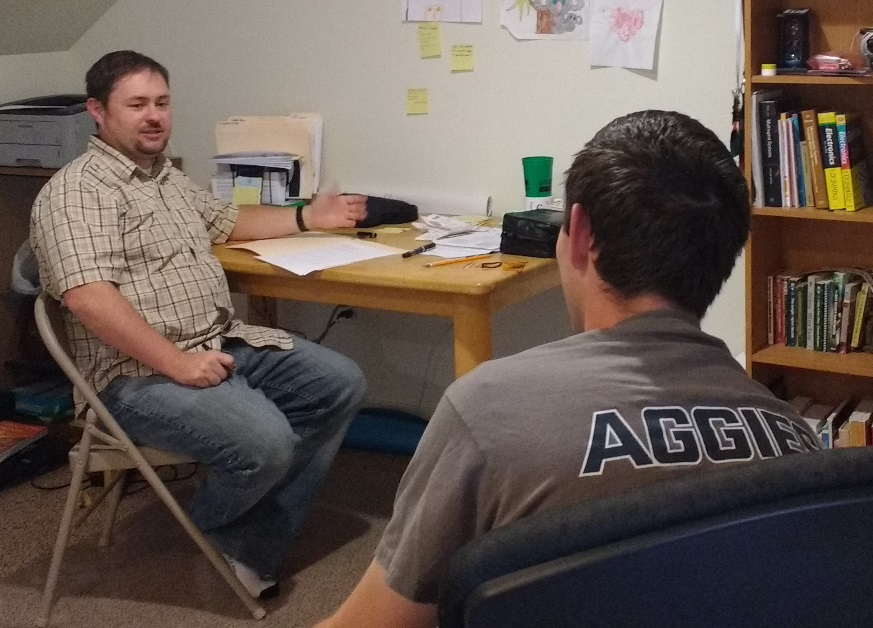
\includegraphics[width=0.9\marginparwidth]{figures/user_study.jpg}
    \caption{A user study was undertaken as one-on-one interviews with 12 subjects.}~\label{fig:marginfig}
  \end{minipage}
\end{marginfigure}



The objective of the interview questions was intended to get an improved
understanding of a typical student's study habits, their prior experience
within a study group setting, as well as their current attitudes in regards
to being part of such a group. The thinking was that if one could
understand the motivation behind a student's need to reach out for help, it
would in turn lead to the best way to create a service that would actually
be accepted and used for their needs.

The interviews were conducted using a semi-structured format with twelve
students attending various universities. While all but one of the students
interviewed were undergraduate students, their level, depth and commitment
to their education seemed to span over a large spectrum of potential users.
The interviews were conducted by each member of the research team and done
one-on-one using various mediums, such as face-to-face interviews in the
subject's home or interviewer's home, over the phone, and via video chat.
The interviews lasted between twenty and thirty minutes, using the same
interview template, yet allowing the interviewer to probe deeper into the
discussion when needed.

\begin{figure}
  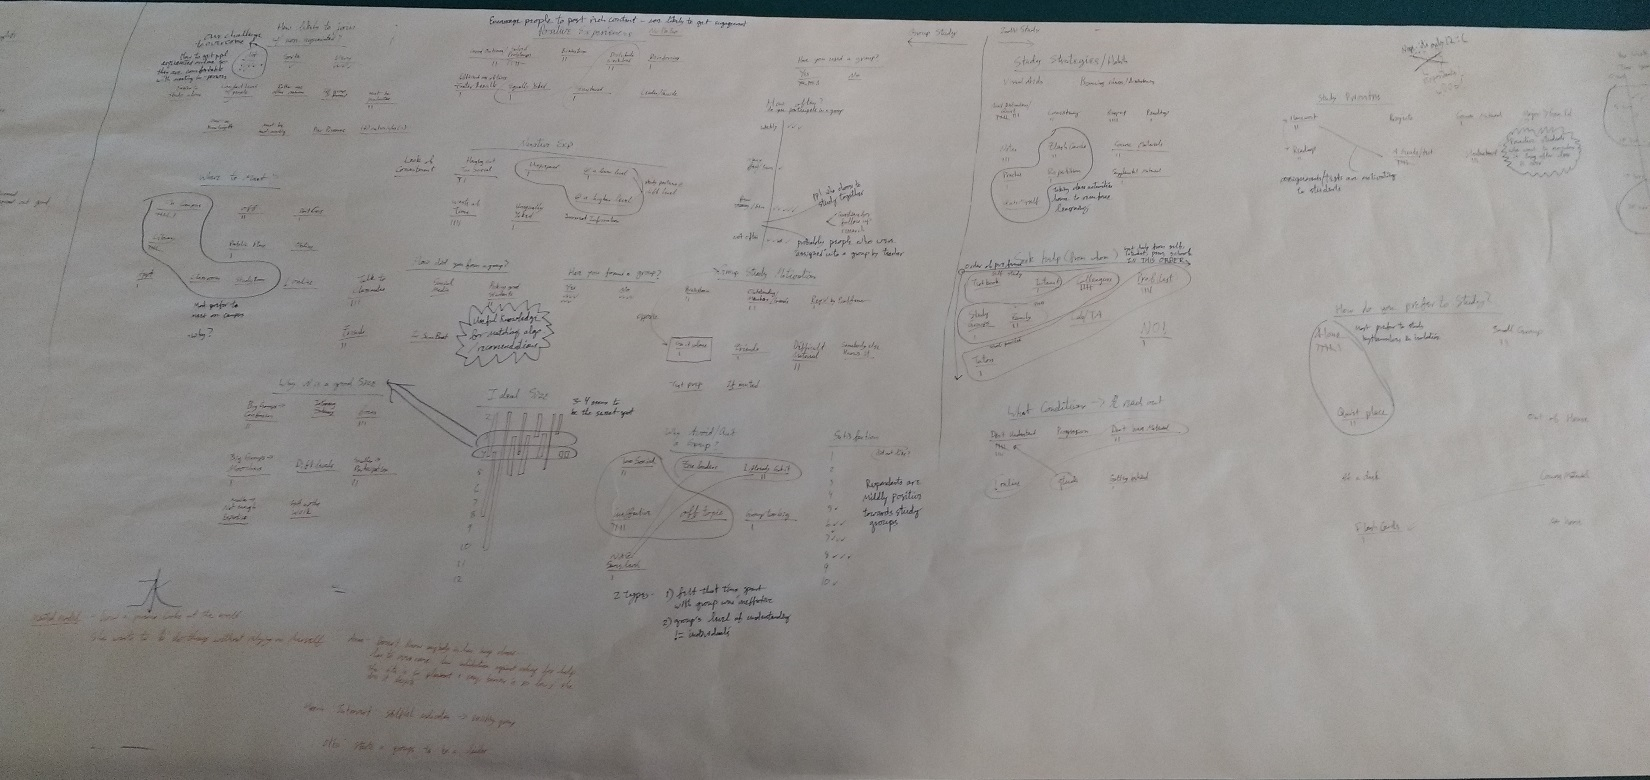
\includegraphics[width=0.9\columnwidth]{figures/affinity_diagram.jpg}
  \caption{Affinity diagram}~\label{fig:sample}
\end{figure}

To aid in understanding the information gathered using this user research,
an affinity diagram was made to group information to help understand the
commonalities among the different participants. In regard to individual
study behavior, individuals tended to spend little to moderate time
studying (less than 10 hours per week) or a large amount of time studying
(15 to 20 hours per week), with none in between. Most of the subjects
preferred to study alone in a quiet location with minimal distractions.
Also, most would not reach out unless they could not understand the
material first; reaching out to material in books or the on the Internet
before searching out friends or classmates direction.

Another finding was that it was agreed that the ideal group size was
between three and four individuals per group. The subjects' rational for
this was due to the negative experiences they had had with larger groups
that suffered from lack of focus or group members' different level of
understanding being too wide to facilitate effective discussion. They also
reported a preference to meet on campus.

However, the greatest finding in this research came about as a result of
those interviewed having had prior study group exposure, with most of it
being due to being assigned to a group by a professor and thus had a
negative experience. Despite this, overall the satisfaction was mildly
positive in regards to their current motivation to study with a group; but
only given the right circumstances within a familiar environment with known
colleagues. This let us to change our focus to getting people into social
situations, to focus more on how to make this tool simple and inviting to
overcome this bias.


\section{Personas and Scenarios}

\subsection{User Personas}

\begin{marginfigure}[-5pc]
  \begin{minipage}{\marginparwidth}
    \centering
  
\includegraphics[width=0.9\marginparwidth]{figures/anna.png}
    \caption{Persona \#1: Anna Redder}~\label{fig:marginfig}
  \end{minipage}
\end{marginfigure}

\begin{marginfigure}[1pc]
  \begin{minipage}{\marginparwidth}
    \centering
  
\includegraphics[width=0.9\marginparwidth]{figures/otto.png}
    \caption{Persona \#2: Otto von Nov }~\label{fig:marginfig}
  \end{minipage}
\end{marginfigure}

\begin{marginfigure}[2pc]
  \begin{minipage}{\marginparwidth}
    \centering
  
\includegraphics[width=0.7\marginparwidth]{figures/marvin.png}
    \caption{Persona \#3: Marvin nivram }~\label{fig:marginfig}
  \end{minipage}
\end{marginfigure}



To aid in structuring this application personas were built to represent
potential users. The personas were derived from the findings of the user
research to represent a typical student. First, a user who is early on in her
education at a school which is far from home, Anna Reeder is still in the
exploring phase of her education as she learns about potential areas of study.
She feels like she has something to prove, motivating the moving out-of-state
to see what else the world has for her, despite numerous unknowns. Secondly,
Marvin Nivram is a student who is further into his undergraduate program, thus
focusing his schedule on the major courses needed to complete his degree. All
the while, he is trying to manage life as a student and husband, living in his
parents' basement, wondering how his uneasiness is social settings is going to
impact him as he seeks a ``real'' job upon graduation. Lastly a foreign graduate
student from Germany named Otto Von Nov has different motivations toward being
a part of a study groups. He willingly seeks them out to aid with the language
barrier that he is dealing with in a new culture and is willing to participate
to develop the skills that will make him successful as a future professor. We
felt that these three personas covered the majority of the demographics of not
only those that we interviewed, but the different social personalities and
living conditions that they are in.

\subsection{Scenarios}

After having the types of people who would use the ``Study Social''
application, scenarios were created to give a better idea of what situations
would drive a user to use the application and how the application would aid
them with their goal. We gave a situation that our user research subjects
indicated was a circumstance which would lead to the need for a study group,
not being able to understand or solve material on their own. We also included a
scenario for those who want to form groups but do not have the tools necessary
to do so. The scenarios were intended to be applied toward a student from any
background falling into the given circumstance, but were applied to the
individual personas for ease. Two of the scenarios were intended to covered the
negative reasons why individuals would stay away from joining groups, then
being placed in a situation where they did not really have any other choice and
used the application to ease social anxiety, or getting the student out of a
bind by waiting too long. The other scenario was to help show that there are
students that recognize the benefits of study groups because they develop
skills that are desirable to employers. Three scenarios seemed to appropriately
convey the meaning of the data that we received in the user research on
overcoming the negative stigma and experiences that are associated with group
studying.



\section{Prototypes}

\subsection{Paper Prototype}

Our design process began by sketching several concepts out on paper. We refined
these sketches through a number of iterations, all the while keeping in balance
competing design considerations.

Working on paper allowed us to quickly explore several diverse structures and
layouts until we found one which we felt would be simple and intuitive. At this
stage we focused on design principles such as ease of exploration and simplicity.
Knowing the time pressures which students face, we aimed to craft an experience
that wold be fun, inviting and, above all, efficient. We reasoned that a
demanding interface would be a turn off to the busy students we are trying to
reach.

\begin{marginfigure}[3pc]
  \begin{minipage}{\marginparwidth}
    \centering
	  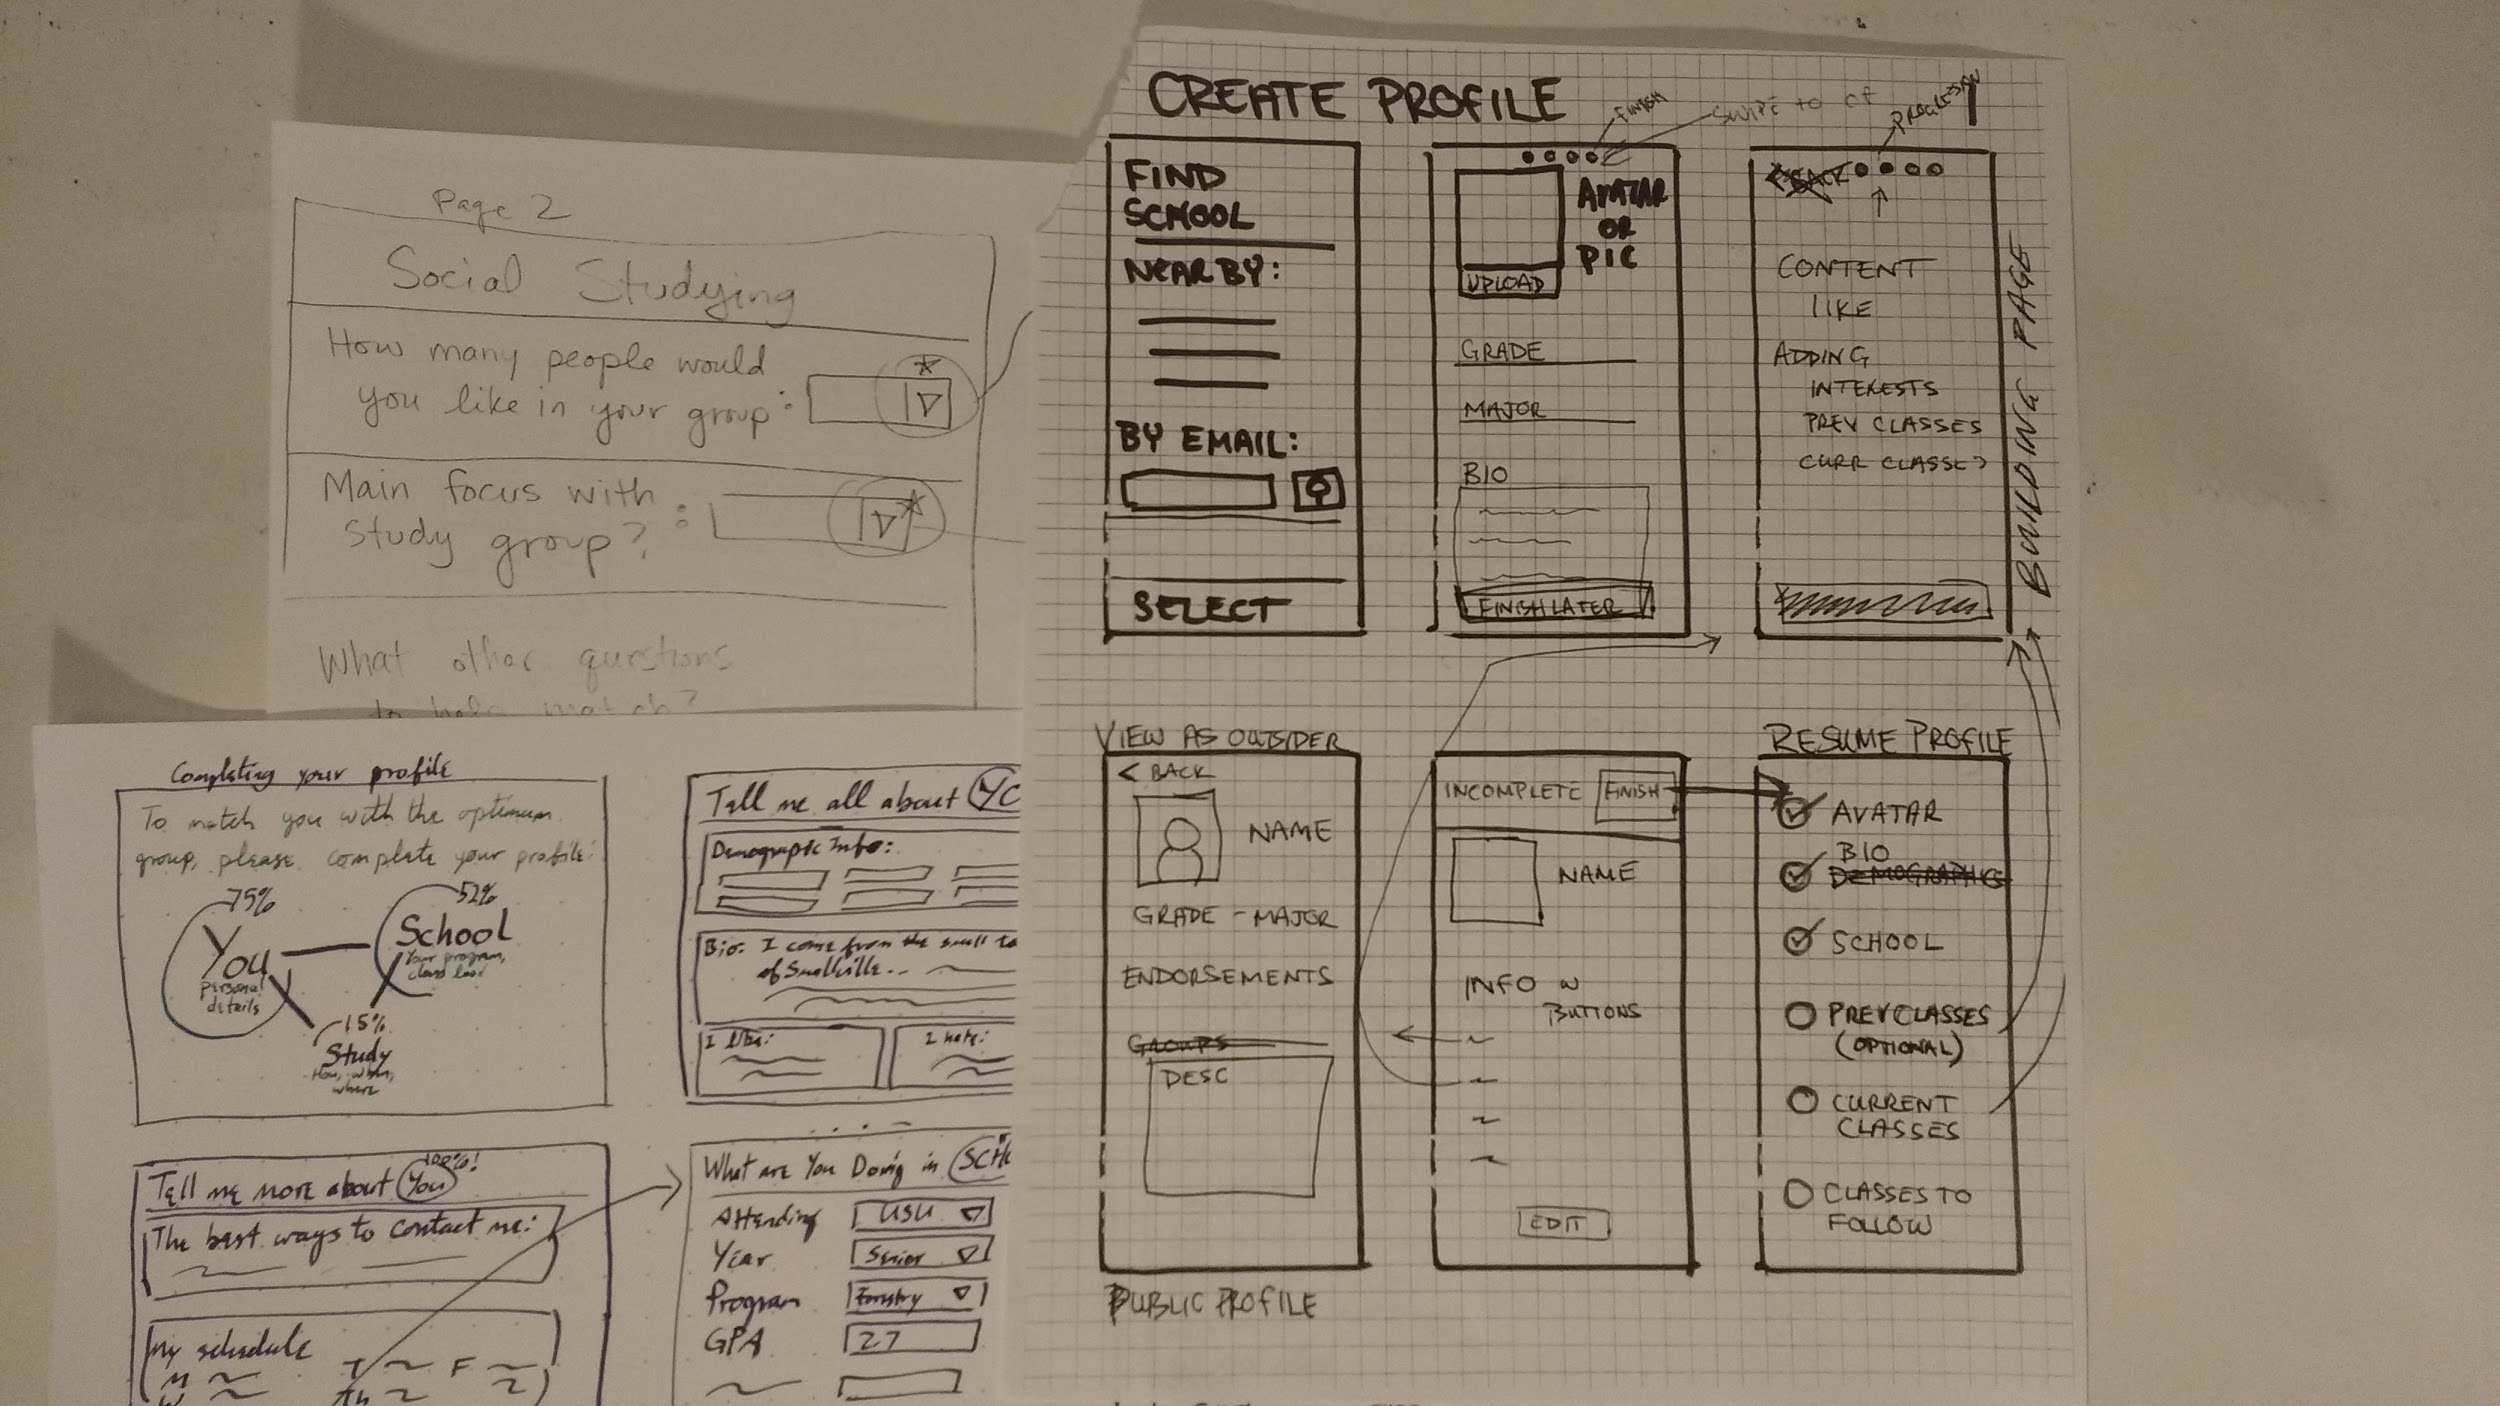
\includegraphics[width=0.7\marginparwidth]{figures/paper_prototype.jpg}
    \caption{Early concept sketches}~\label{fig:marginfig}
  \end{minipage}
\end{marginfigure}



\subsection{Digital Prototype}

\begin{marginfigure}[0pc]
	\begin{minipage}{\marginparwidth}
		\centering
		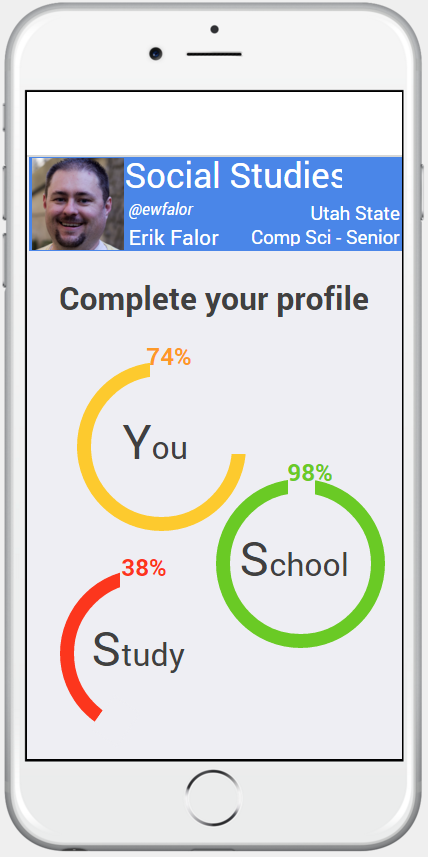
\includegraphics[width=0.9\columnwidth]{figures/prototype1.png}
		\caption{Profile landing page of the initial prototype}~\label{fig:prototype}
	\end{minipage}
\end{marginfigure}


After settling on a concept we created a digital prototype using the JustInMind Prototyping
tool~\cite{justinmind}. This software program enabled our team to create a hi-fidelity interactive
prototype with the ease of making a drawing. The JustInMind Prototyping tool supplies built-in
templates for designing both desktop and mobile applications. Realizing that digital content is
mostly consumed on mobile devices, we focused our efforts on creating a mobile prototype. With this
tool we were quickly able to produce a working prototype which brought to life our paper drawings.


\subsection{Cognitive Walk-through}

Members of our team guided four participants through a cognitive walk-through
evaluation. Participants were asked to complete a few simple, pre-defined tasks
using the digital prototype from a web browser. Having an interactive
web-based prototype made administering the cognitive walk-through simple owing
to the fact that our test subjects were already comfortable with the concept of
a webpage and could begin tackling their assigned tasks with minimal prompting.

The cognitive walk-through revealed weaknesses in our design which we had theretofore been blind to.
One such revelation was that our navigation scheme was insufficient and inconsistent, leaving users
lost and confused.

This design deficit followed from our understanding of how a paper prototype
ought to be designed. Looking back, it is clear that we had come to envision
the application as a sequence of hyperlinked pages, one screen in size instead
of imagining it as a unified, continuous flow.  Navigation was unnecessarily
difficult because it wasn't always clear on which screen a piece of desired
information was located, nor was it obvious how to reach a desired destination
from the user's current screen.

Another issue reported by a majority of participants was inadequate feedback.
An oft-cited complaint was that after painstakingly entering data into the
mobile application via an on-screen keyboard, there was no "save" button
provided. Navigating back to the previous screen did not reassure the user that
their data was saved. Nor was there any indication of an autosave feature.
Because of this users sought in vain for the missing button and were reluctant
to leave the page containing the text-entry forms.



\subsection{Heuristic evaluation}

Following the cognitive walk-through our team performed a heuristic evaluation on the most important
functions of the application. Of the ten design heuristics under consideration, two repeatedly came
up as problematic to our prototype. These were ``User control and freedom'' and ``consistency and
standards''. The aforementioned navigation confusion along with the lack of a save button were the
biggest drivers of the former heuristic. The latter was exemplified by our inconsistent use of
navigation hints and our over-complicated search interface.



\section{Usability Testing}

The result of the foregoing evaluation activities was a bottom-up redesign of
our application prototype which was prepared for a usability testing activity.
This usability testing of the application was performed with the assistance of
five volunteers, drawn from the pool of participants of our prior research
activities. As with the cognitive walk-through, the usability testing activity
was performed using the JustInMind Prototyping tool~\cite{justinmind}.  These
users were able to judge the difference between the initial and improved
prototype, and all agreed that the new prototype addressed their concerns.

Users performed a sequence of tasks including creating and populating a
personal profile, finding an existing study group and creating a new study
group. As participants completed these tasks they vocalized their thoughts and
frustrations so that we cold better understand the thought process of a typical
user.


\marginpar{
	\vspace{-80pt}
	\fbox {
		\begin{minipage}{0.925\marginparwidth}
			\textbf{Usability Testing Tasks}
			\begin{itemize}
				\item	Create account
				\item	Edit Profile
				\item	Make Profile Private
				\item	Find and Join Group
				\item	Create new group
			\end{itemize}
		\end{minipage}
	}
}

\begin{marginfigure}[23pt]
  \begin{minipage}{\marginparwidth}
    \centering
	  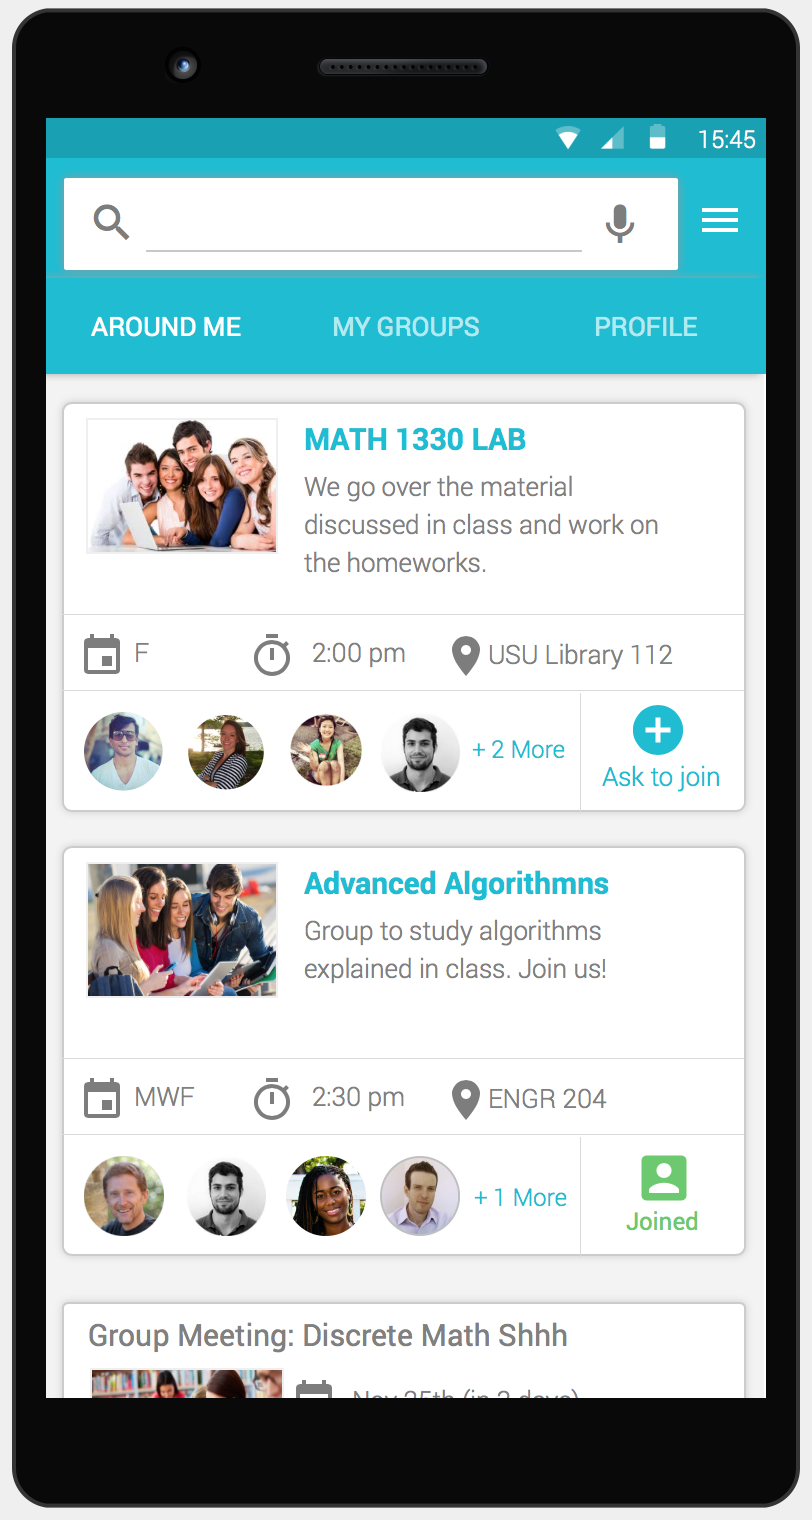
\includegraphics[width=0.7\marginparwidth]{figures/beta_prototype.png}
    \caption{Final prototype}~\label{fig:marginfig}
  \end{minipage}
\end{marginfigure}





\section{Conclusion}

Understanding the barriers keeping students from enjoying effective group study
sessions helped our team create the Study Social application. Our initial group of
interviewees who expressed negative feelings towards group study later remarked
that they would definitely use the product our final prototype represented.
Evolving our idea from a simple tutor-student matching application to a
complete group collaboration study application with chat and file uploads was a
iterative process led by research.  Study Social is positioned to fill a niche
in the market between a social forming application and a collaboration tool.
Students can overcome the initial barriers of forming functioning study groups
and improve confidence, understanding, accuracy, and overcome frustration by
working together on difficult material.        


\section{Acknowledgements}

We are grateful to all of the participants who
volunteered through interviews, cognitive walk-throughs, usability tests and in
other activities. Their input was invaluable and really helped this project
take shape.  We owe a debt of gratitude to our helpful and enthusiastic mentor
and advisor, Dr. Amanda Hughes. We could never have created such a successful
prototype without her brilliant insight and helpful advice.  Some of the
references cited in this paper are included for illustrative purposes only.



\balance{}

% \bibliographystyle{ACM-Reference-Format-Journals}
\bibliographystyle{SIGCHI-Reference-Format}
% \bibliographystyle{acm}
\bibliography{Team-FTW-Report}

\end{document}

%%% Local Variables:
%%% mode: latex
%%% TeX-master: t
%%% End:
